\documentclass[11pt, a4paper]{article} % setsfont size and layout

%% required packages %%

\usepackage[margin=2.5cm]{geometry} % margins
\usepackage[english]{babel} % language (replace with german or ngerman for german texts)
\usepackage[utf8]{inputenc} % Umlaute
\usepackage{amsmath}		% math formulas
\usepackage{graphicx}		% graphics
\usepackage{fancyhdr}		% header and footer on every page
\usepackage{setspace}		% line space (e.g. \singlespacing, \onehalfspacing or \doublespacing)
\usepackage{xcolor}
\usepackage{subcaption}
\usepackage{pdflscape}
\usepackage{rotating}
\usepackage[boxruled, lined, vlined]{algorithm2e}
\SetKwFor{For}{for (}{) $\lbrace$}{$\rbrace$}
\usepackage{multicol}



\begin{document}
	
%% Some more settings %%
	
\setlength{\parindent}{0pt} % first line in paragraph will not be indented
\onehalfspacing				% 1.5 line spacing
%\thispagestyle{empty}		% no header and page number on first page


%% Header on first page with course information etc. %%
\begin{tabular}{p{15.5cm}}
	{\large \textbf{Inrobin}} \\
	Gareth W. Peters  \\ 
	Dorota Toczydłowska\\
	Marta Campi\\
	\hline
	\\
\end{tabular}

\vspace*{0.3cm}				% vertical space between header on top of the page and main heading


\begin{center}
	{\LARGE \textbf{Experiment one:}}
	\vspace{2mm}	
\end{center} 



\section*{Calibration of the Hyperparameters to assess performances of the KTA}

Set the notation of this experiment as follows:

$\Omega_{test}$ - the set with $M_{test}$ parameters\\
$\Omega_{true}$ - the set with $M_{true}$ parameters\\
Let $\Psi_{test}^{(i)}$ be an $i$th parameter from $\Omega_{test}$\\
Let $\Psi_{true}^{(j)}$ be an $j$th parameter from $ \Omega_{true}$\\
$k(\cdot, \cdot;\Psi)$ a kernel function from parameterized by the parameter $\Psi$,  $k: \mathcal{R} \times \mathcal{R} \rightarrow \mathcal{R}$\\ 
Let $\mathbf{t}$ be a $1\times N$ vector of real numbers\\
$\mathbf{K}_{true} = k(\mathbf{t}, \mathbf{t};\Psi = \Psi_{true})$\\
$\mathbf{K}_{test} = k(\mathbf{t}, \mathbf{t};\Psi = \Psi_{test})$

$i \in \Big\{ 1, \cdots, M_{test} \Big\}$, $j \in \Big\{ 1, \cdots, M_{true} \Big\}$\\
$\Psi_{test}^{(i)} = \Omega_{true} [i]$\\
$A(K1,K2) : = 2 - \left\| \frac{K_1}{\left\| K_1 \right\|_F} - \frac{K_2}{\left\| K_2 \right\|_F} \right\|_F$\\
$m \in {1, \cdots, M}$

\hfill

\begin{algorithm}[H]


\label{algo_exp1}
\caption{Algorithm}

\BlankLine
\addtolength\linewidth{-12ex}

\KwIn{Define $k, \Omega_{true}, \Omega_{test}, \mathbf{t}$\\
Set $i ,j,m$}
%\KwOut{CKTA between $\mathbf{S}_{N \times N}^{(m)}$ and Kernel Gram Matrix $\mathbf{K}_{(test,i)}$ }

\begin{enumerate}

\item Evaluate the Gram Matrix $\mathbf{K}_{(true,j)} = k(\mathbf{t},\mathbf{t}; \Psi_{(true,j)})$ parametrized by the $j$th parameter from $\Omega_{true}$ \\

\item Simulate $\mathbf{y}^{(m)} \sim \mathcal{N}(0, \mathbf{K}_{(true,j)})$ be an N dimensional vector\\
\item Compute the sample covariance matrix given by $\mathbf{S}_{N \times N}^{(m)} = \mathbf{y}^{(m) T} \mathbf{y}^{(m)}$ \\

\item Evaluate the Gram Matrix $\mathbf{K}_{(test,i)} = k( \mathbf{t}, \mathbf{t}; \Psi_{(test,i)})$ parametrized by the $i$th parameter from $\Omega_{test}$ \\

\item Compute the CKTA given by $a_{j,i,m} = A(\mathbf{S}_{N \times N}^{(m)},\mathbf{K}_{(test,i)} )$

\end{enumerate}

\end{algorithm}


\hfill
\newpage



\begin{algorithm}[H]


\label{algo_exp1}
\caption{Algorithm}

\BlankLine
\addtolength\linewidth{-12ex}

\KwIn{Define $k, \Omega_{true}, \Omega_{test}, \mathbf{t}$}
%\KwOut{CKTA between $\mathbf{S}_{N \times N}^{(m)}$ and Kernel Gram Matrix $\mathbf{K}_{(test,i)}$ }

\For{$j = 1:M_{true}$}{

Evaluate $\mathbf{K}_{(true,j)} = k(\mathbf{t},\mathbf{t}; \Psi_{(true,j)})$\\

\For{$m=1:M$}{
Simulate $\mathbf{y}_{1 \times N}^{(m)} \sim \mathcal{N}(\mathbf{0}, \mathbf{K}_{(true,j)})$\\
Compute  $\mathbf{S}_{N \times N}^{(m)} = \mathbf{y}^{(m) T} \mathbf{y}^{(m)}$ \\

\For{$i = 1:M_{test}$}{

Evaluate the Gram Matrix $\mathbf{K}_{(test,i)} = k( \mathbf{t}, \mathbf{t}; \Psi_{(test,i)})$ parametrized by the $i$th parameter from $\Omega_{test}$ \\

Compute the CKTA given by $a_{j,i,m} = A(\mathbf{S}_{N \times N}^{(m)},\mathbf{K}_{(test,i)} )$

}

}
}
\end{algorithm}


\textcolor{red}{DOROTA:\\
way of presenting\\
which one do we want\\
difference psi? check together}



\newgeometry{left=2.3cm,bottom=0.1cm} 
\begin{landscape}
\begin{figure}
\begin{subfigure}{\textwidth}
  \centering
  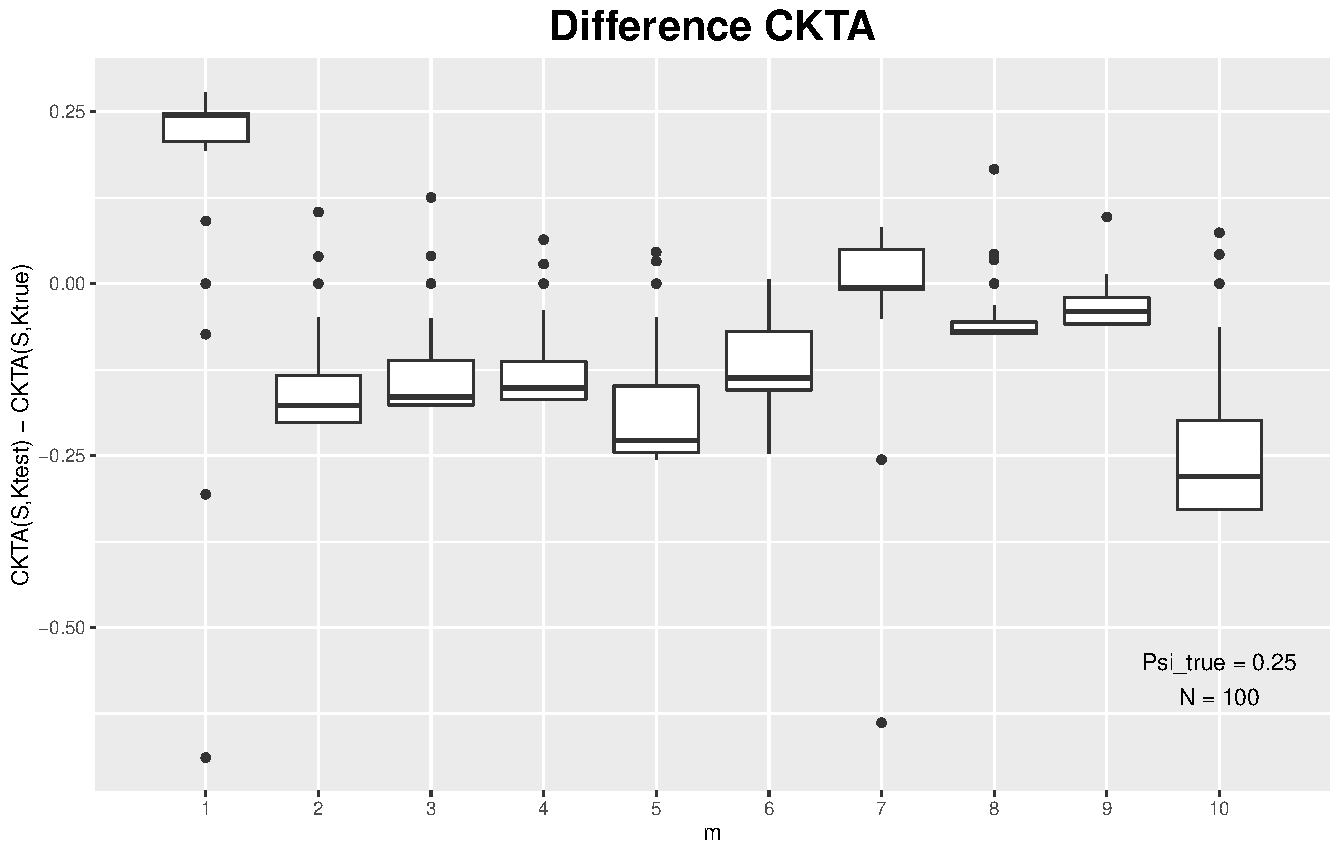
\includegraphics[width=.8\linewidth]{dif_ckta_psi_025.pdf}
%  \caption{1a}
  \label{fig:sfig1}
\end{subfigure}%
\begin{subfigure}{\textwidth}
  \centering
  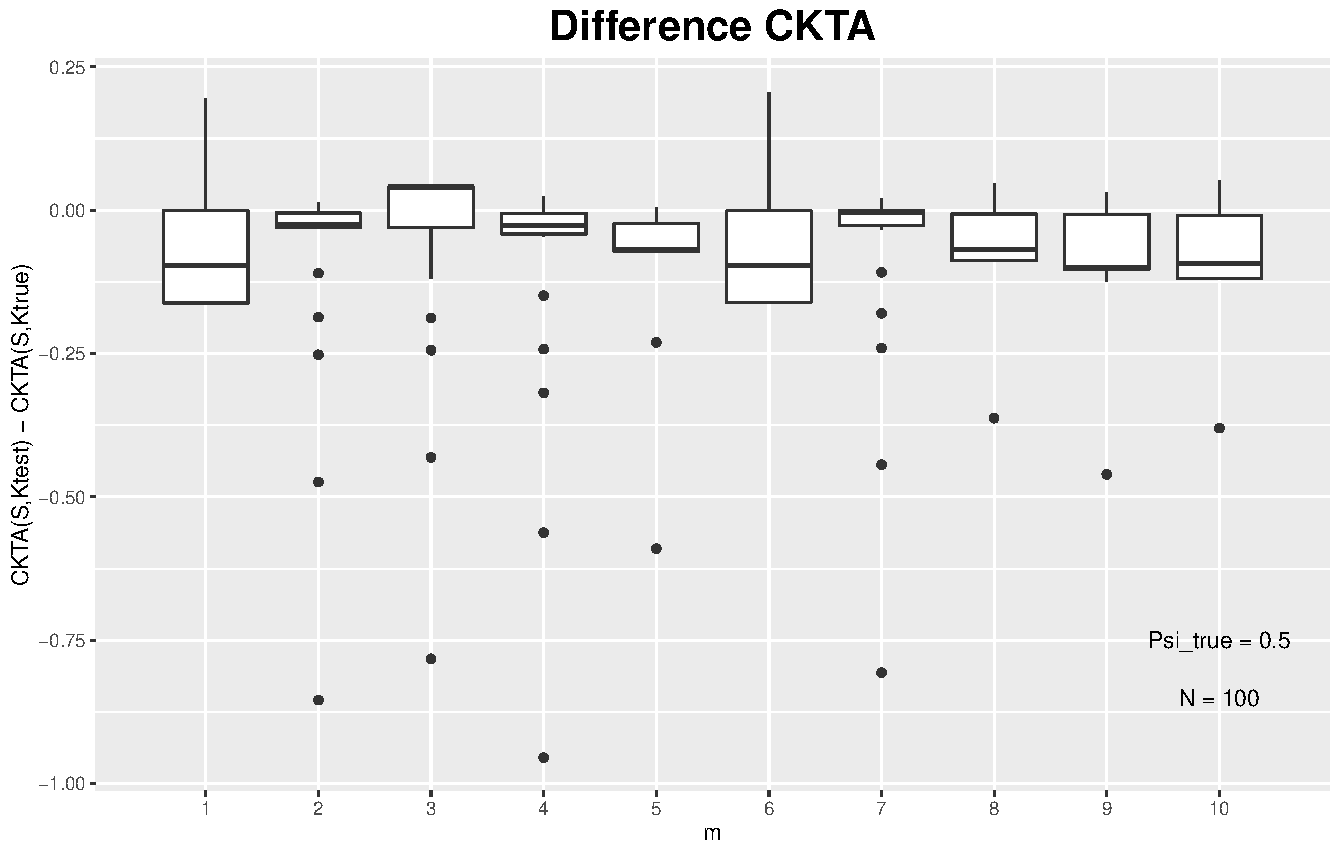
\includegraphics[width=.8\linewidth]{dif_ckta_psi_050.pdf}
%  \caption{1b}
  \label{fig:sfig2}
\end{subfigure}\\

\begin{subfigure}{\textwidth}
  \centering
  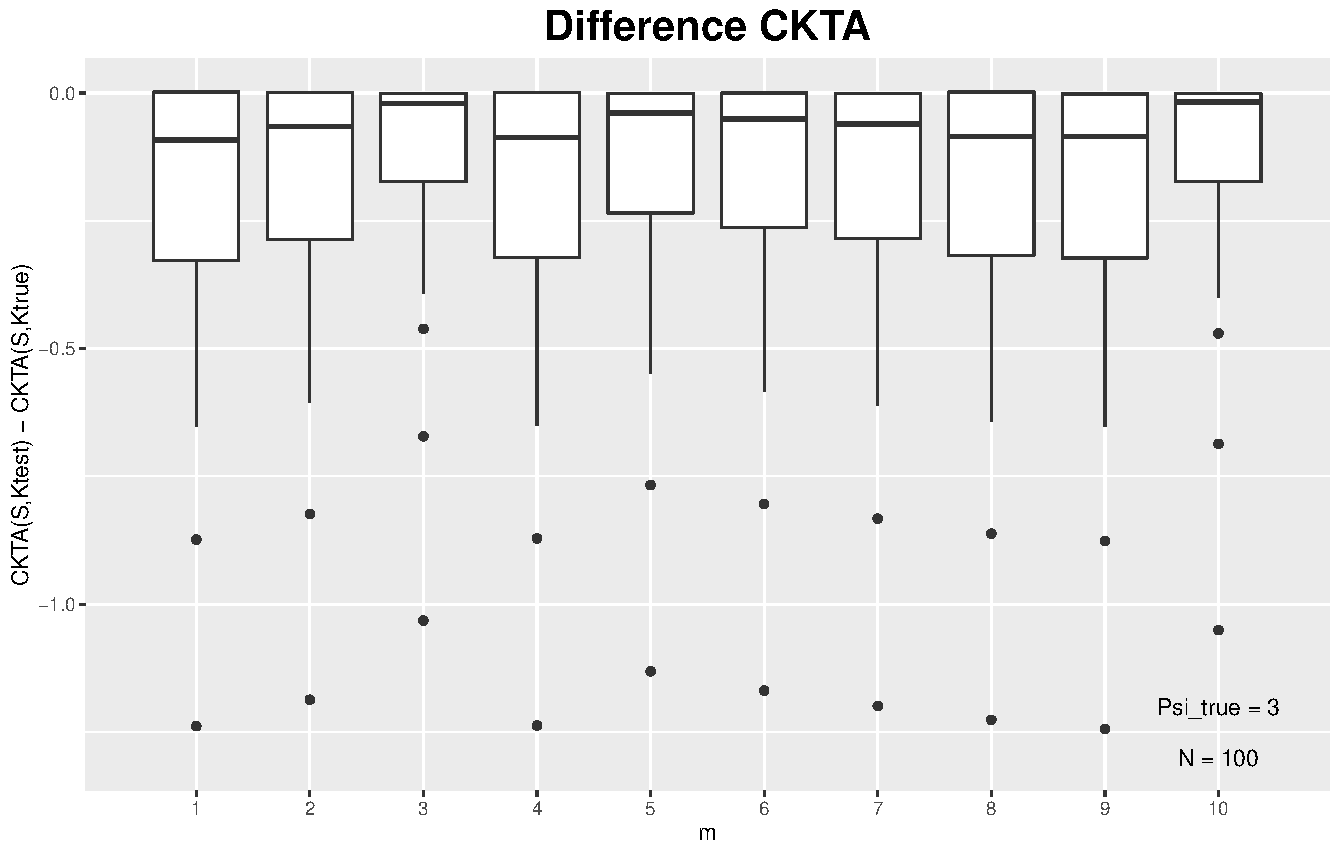
\includegraphics[width=.8\linewidth]{dif_ckta_psi_3.pdf}
%  \caption{1a}
  \label{fig:sfig1}
\end{subfigure}%
\begin{subfigure}{\textwidth}
  \centering
  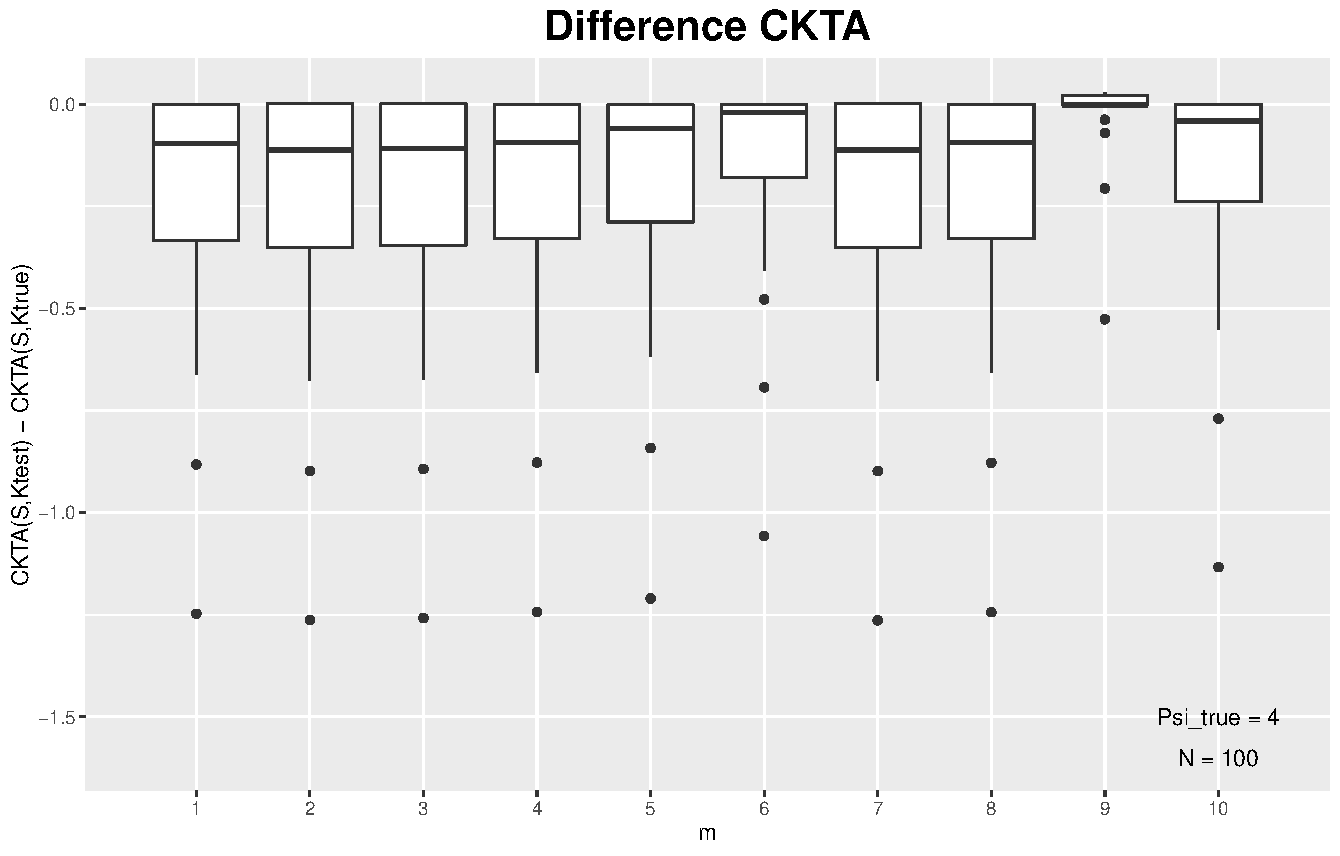
\includegraphics[width=.8\linewidth]{dif_ckta_psi_4.pdf}
%  \caption{1b}
  \label{fig:sfig2}
\end{subfigure}%
\caption{Boxplot of CKTA differences with $m = 10$, $N = 100$. From top left to bottom right $\Psi_{true} = 0.25, 0.5, 3,4$}
\end{figure}
\end{landscape}

\restoregeometry

\newgeometry{left=2.3cm,bottom=0.1cm} 
\begin{landscape}
\begin{figure}
\begin{subfigure}{\textwidth}
  \centering
  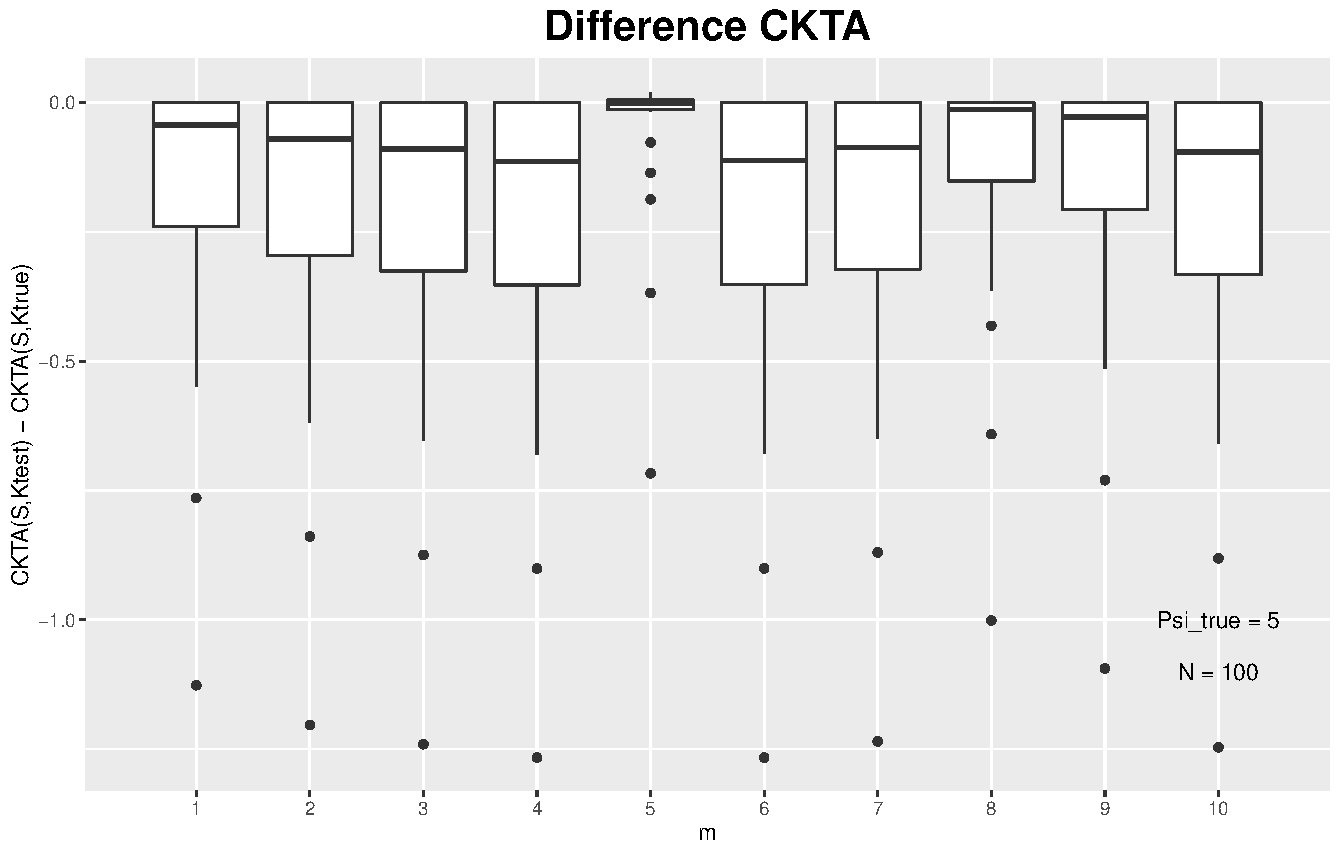
\includegraphics[width=.8\linewidth]{dif_ckta_psi_5.pdf}
%  \caption{1a}
  \label{fig:sfig1}
\end{subfigure}%
\begin{subfigure}{\textwidth}
  \centering
  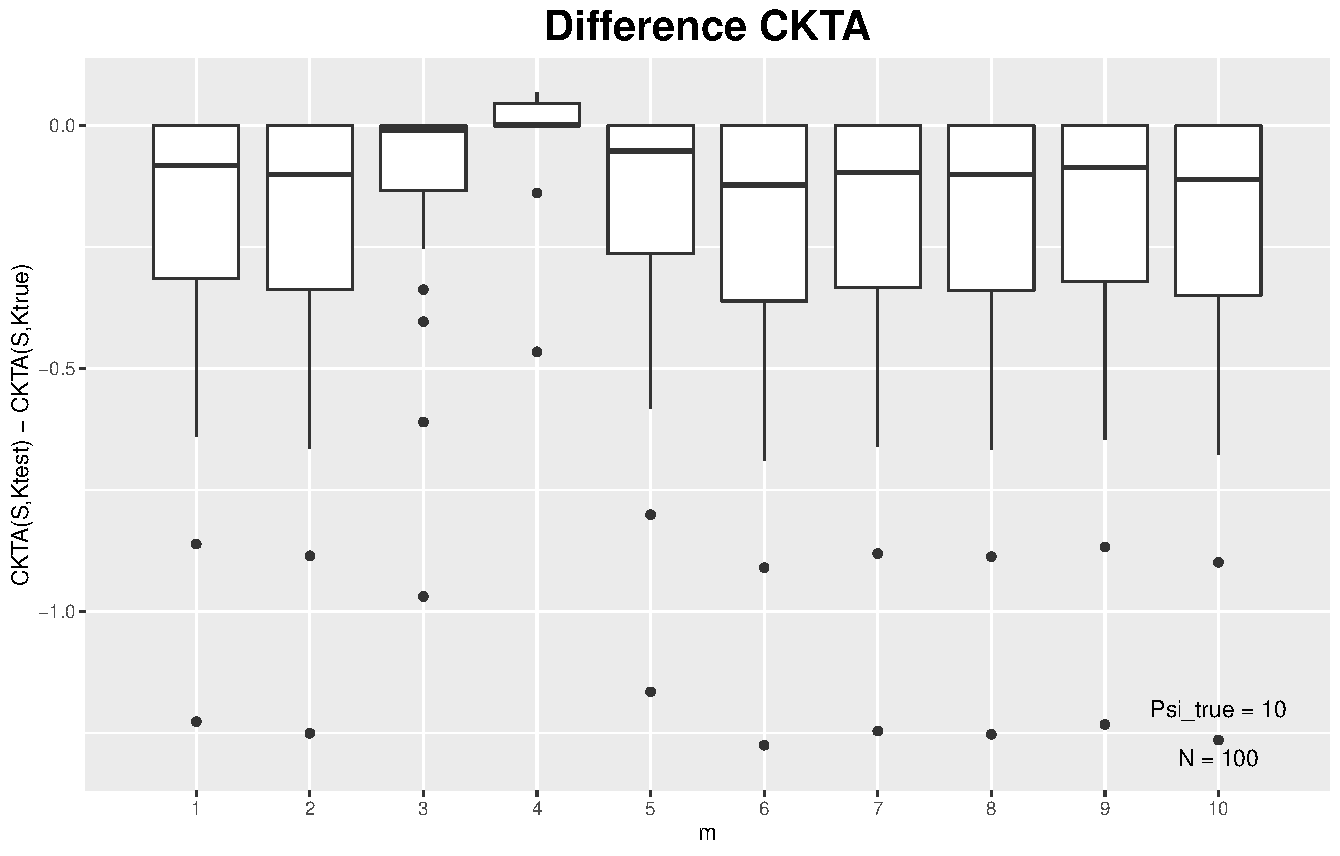
\includegraphics[width=.8\linewidth]{dif_ckta_psi_10.pdf}
%  \caption{1b}
  \label{fig:sfig2}
\end{subfigure}\\

\begin{subfigure}{\textwidth}
  \centering
  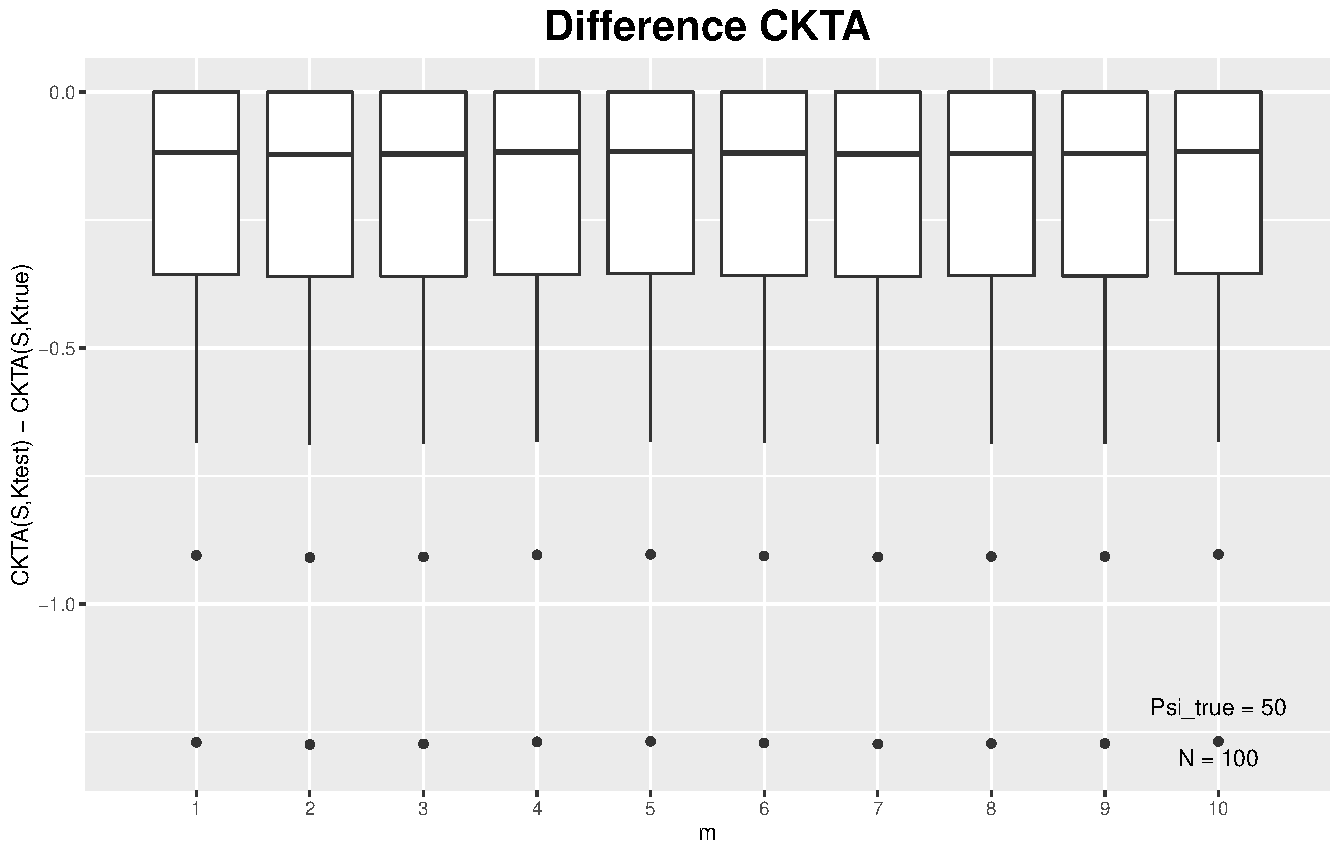
\includegraphics[width=.8\linewidth]{dif_ckta_psi_50.pdf}
%  \caption{1a}
  \label{fig:sfig1}
\end{subfigure}

\caption{Boxplot of CKTA differences with $m = 10$, $N = 100$. From top left to bottom left $\Psi_{true} = 5, 10, 50$}
\label{fig1}
\end{figure}

\end{landscape}

\restoregeometry



\newgeometry{left=2.3cm,bottom=0.1cm} 
\begin{landscape}
\begin{figure}
\begin{subfigure}{\textwidth}
  \centering
  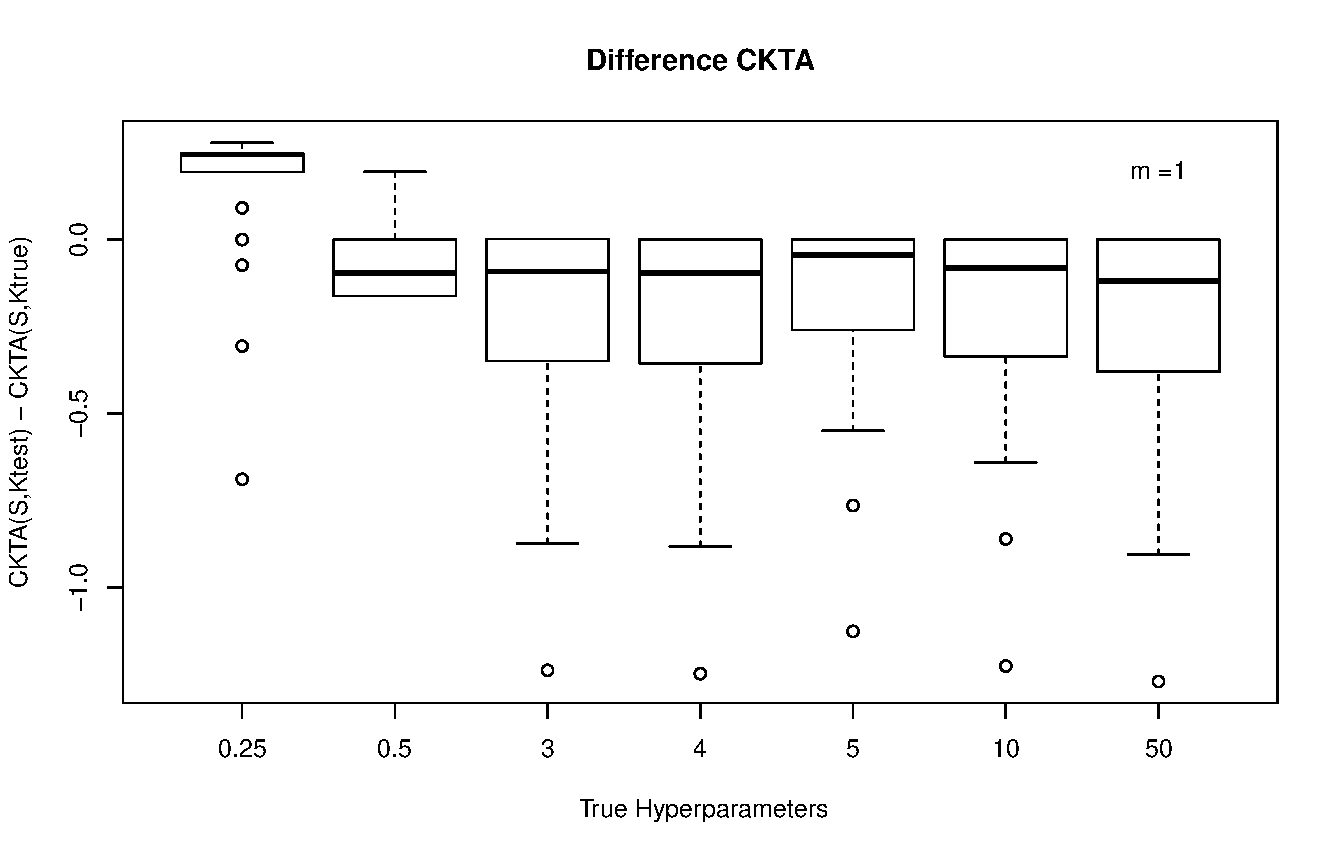
\includegraphics[width=.8\linewidth]{dif_ckta_m_1.pdf}
%  \caption{1a}
  \label{fig:sfig1}
\end{subfigure}%
\begin{subfigure}{\textwidth}
  \centering
  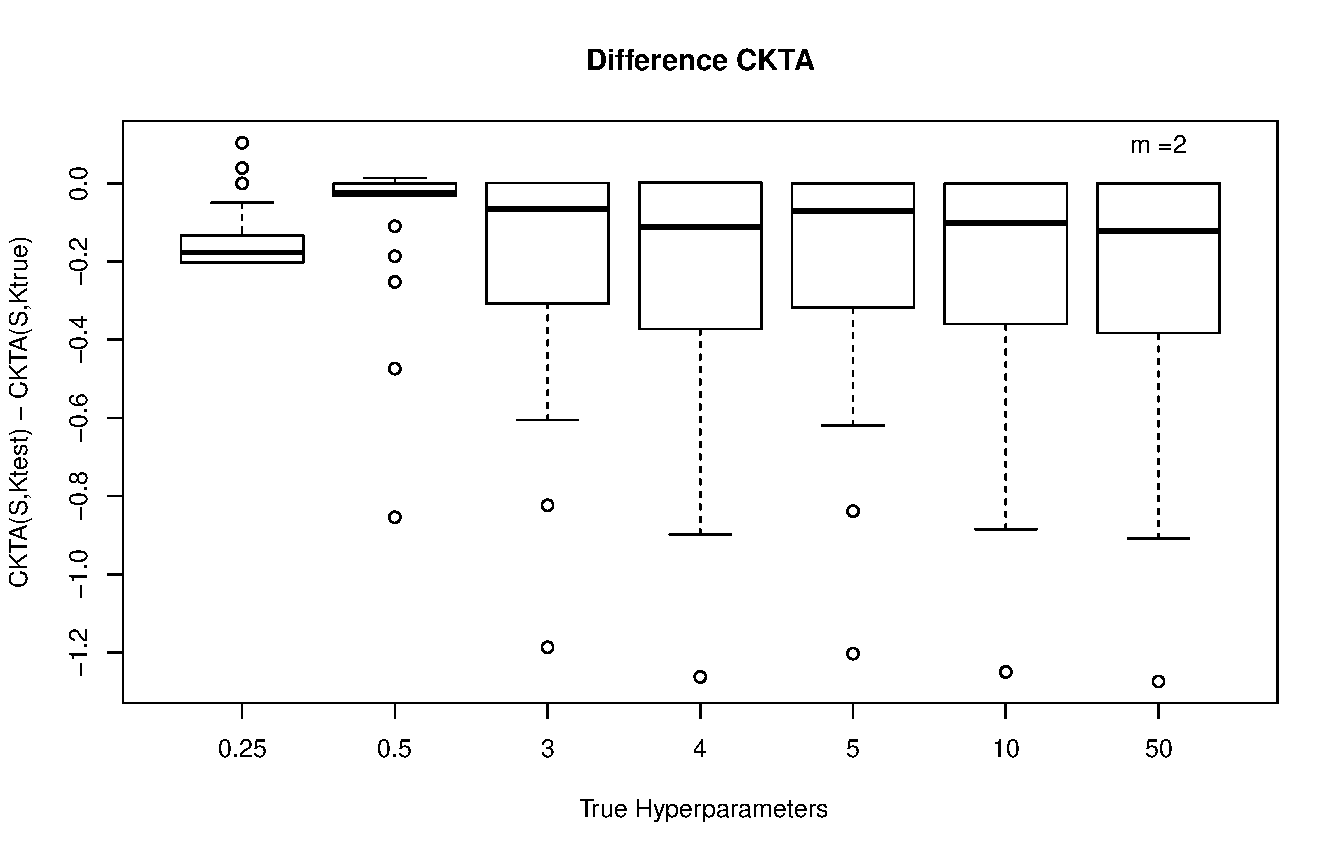
\includegraphics[width=.8\linewidth]{dif_ckta_m_2.pdf}
%  \caption{1b}
  \label{fig:sfig2}
\end{subfigure}\\

\begin{subfigure}{\textwidth}
  \centering
  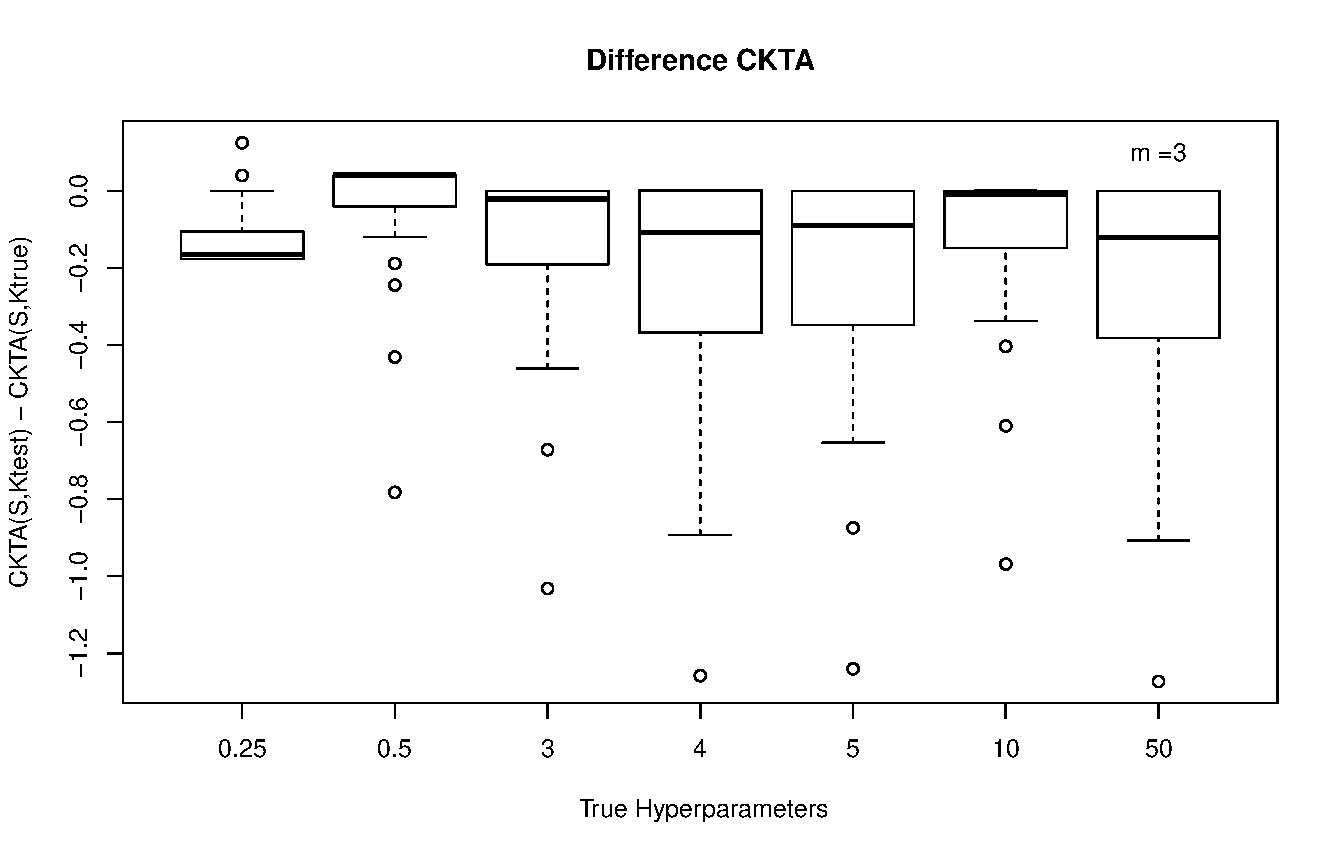
\includegraphics[width=.8\linewidth]{dif_ckta_m_3.pdf}
%  \caption{1a}
  \label{fig:sfig1}
\end{subfigure}%
\begin{subfigure}{\textwidth}
  \centering
  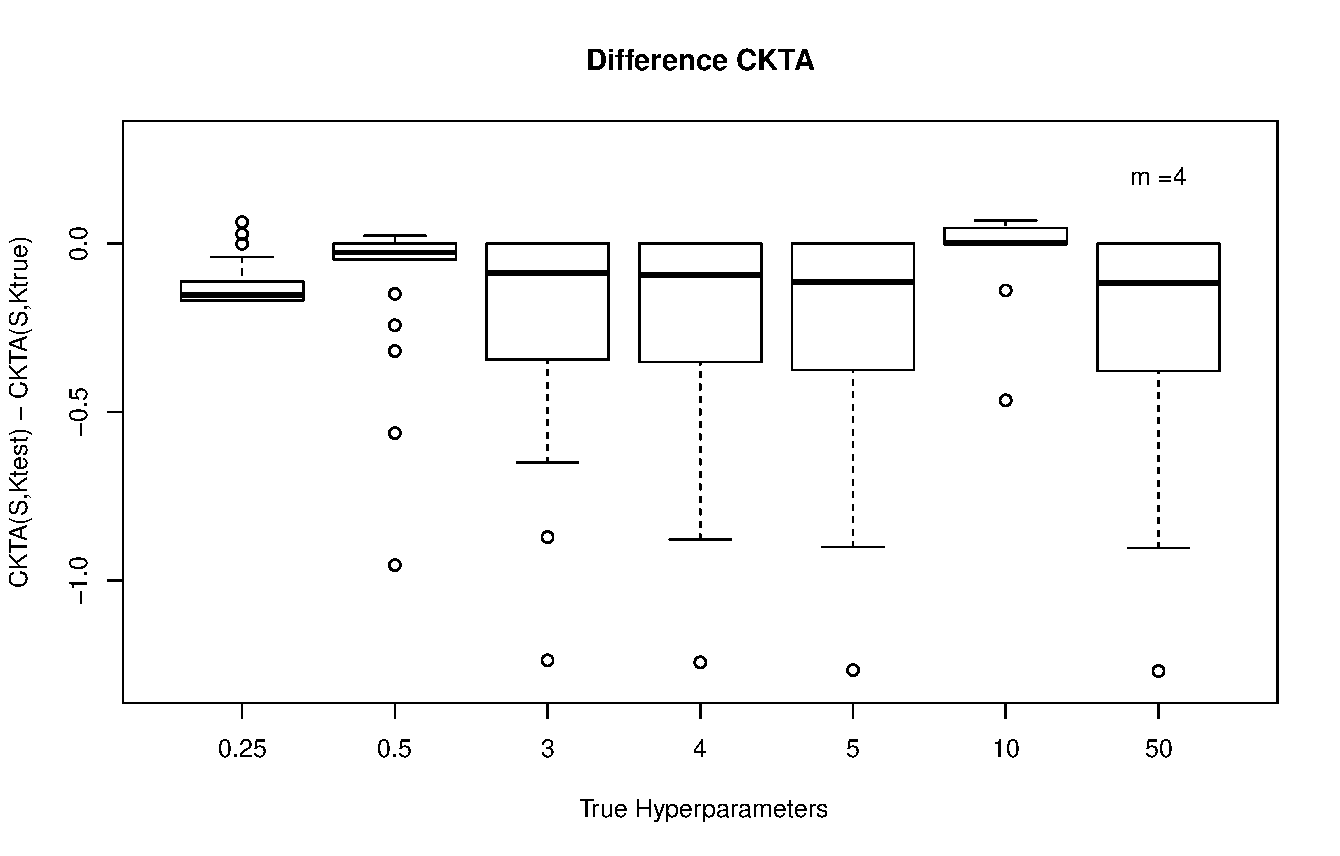
\includegraphics[width=.8\linewidth]{dif_ckta_m_4.pdf}
%  \caption{1a}
  \label{fig:sfig1}
\end{subfigure}


\label{fig1}
\end{figure}

\end{landscape}

\restoregeometry



\newgeometry{left=2.3cm,bottom=0.1cm} 
\begin{landscape}
\begin{figure}
\begin{subfigure}{\textwidth}
  \centering
  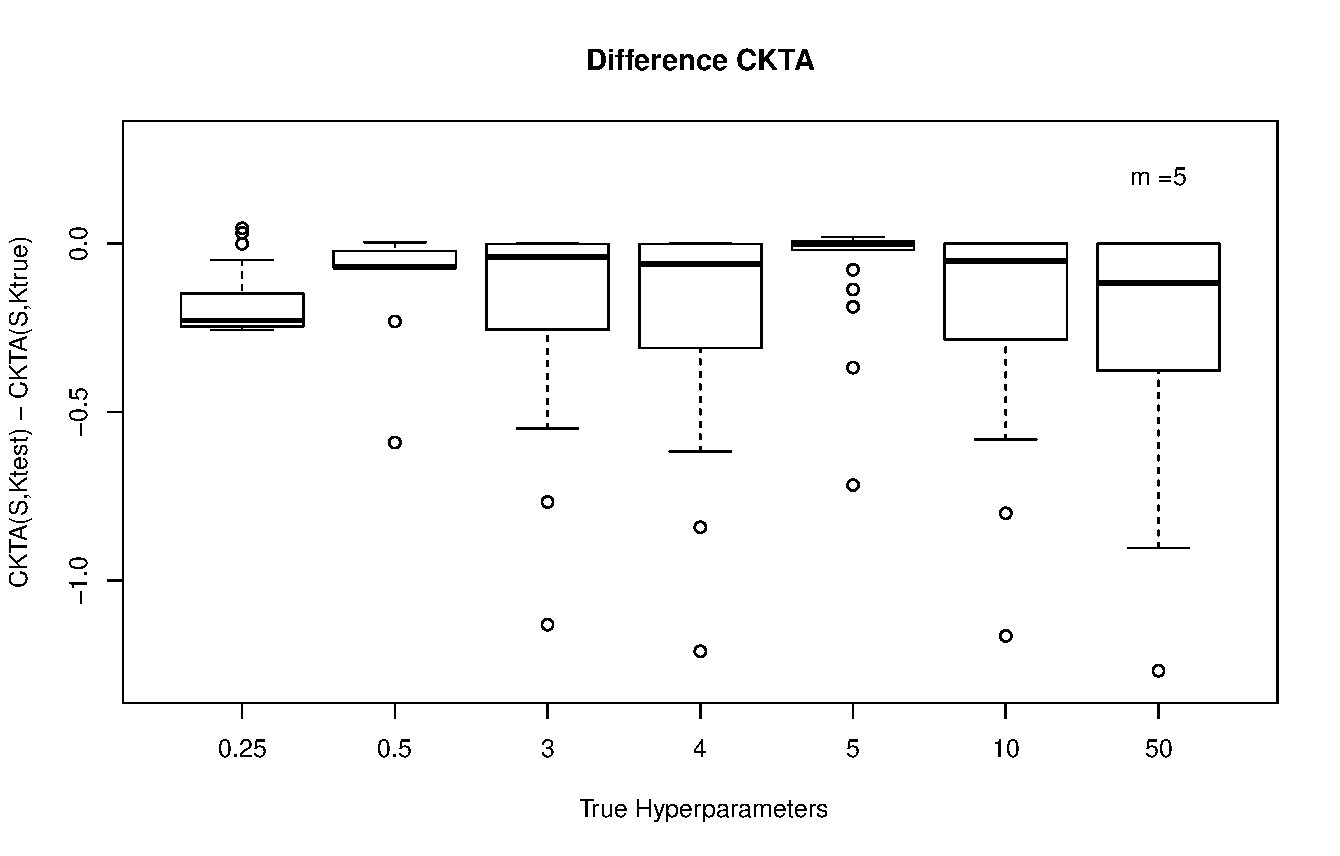
\includegraphics[width=.8\linewidth]{dif_ckta_m_5.pdf}
%  \caption{1a}
  \label{fig:sfig1}
\end{subfigure}%
\begin{subfigure}{\textwidth}
  \centering
  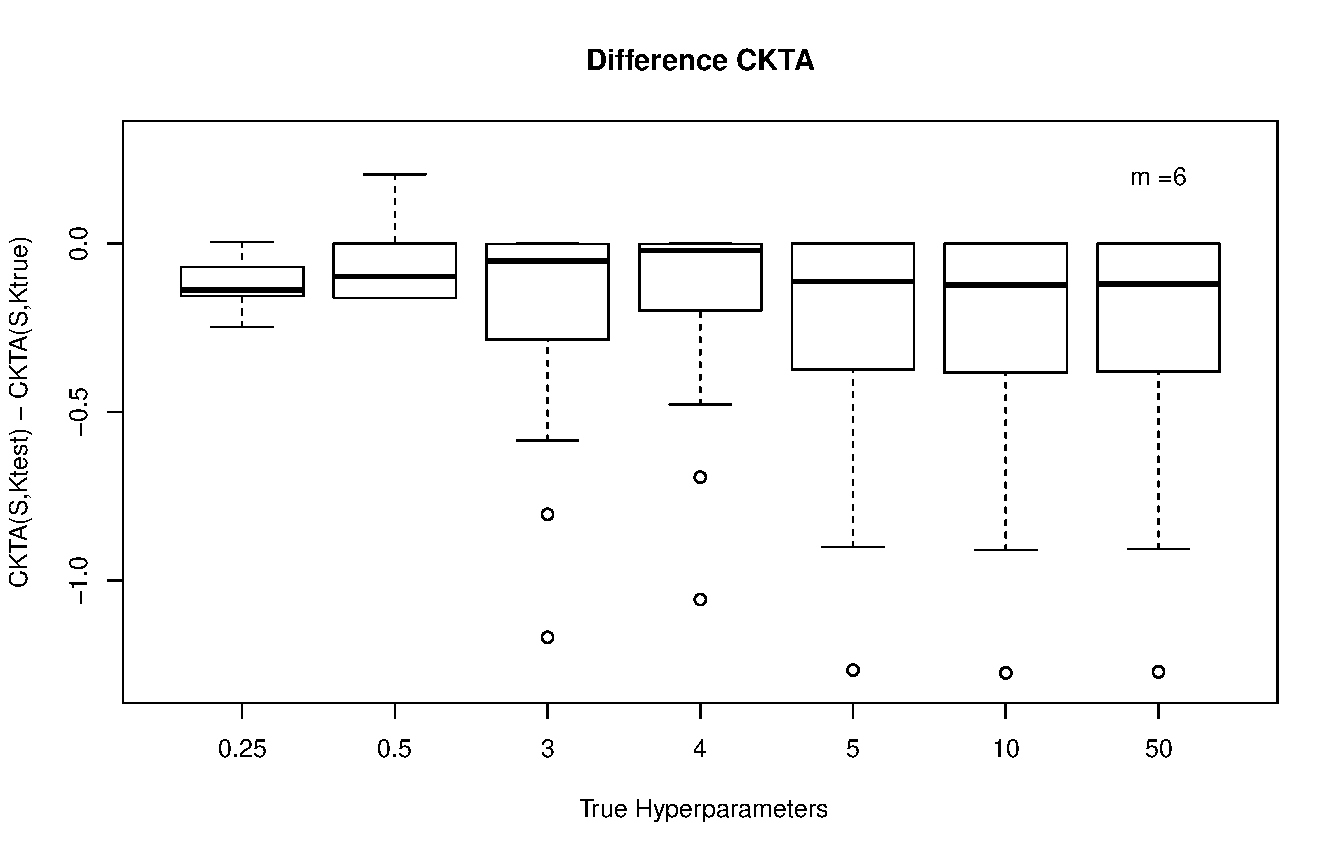
\includegraphics[width=.8\linewidth]{dif_ckta_m_6.pdf}
%  \caption{1b}
  \label{fig:sfig2}
\end{subfigure}\\

\begin{subfigure}{\textwidth}
  \centering
  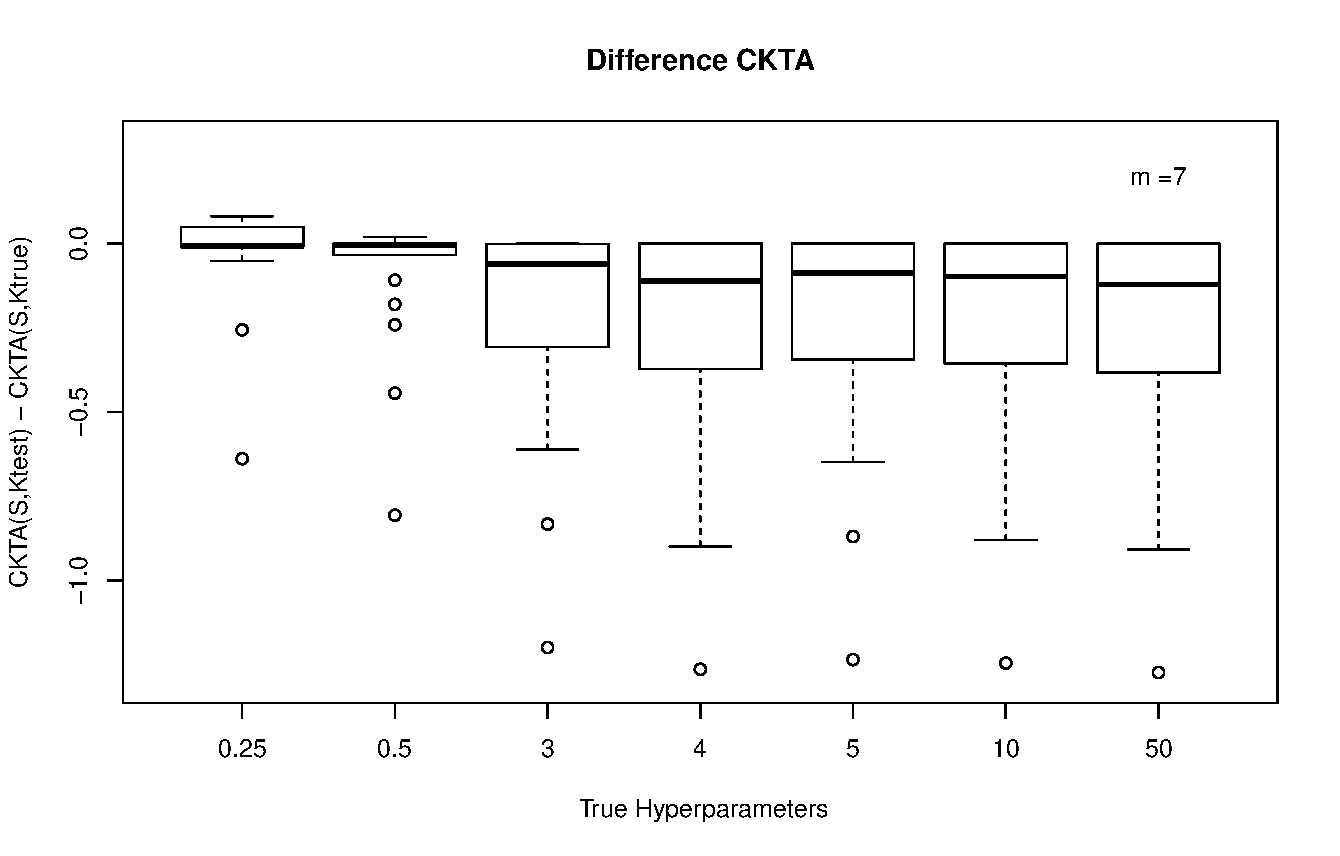
\includegraphics[width=.8\linewidth]{dif_ckta_m_7.pdf}
%  \caption{1a}
  \label{fig:sfig1}
\end{subfigure}%
\begin{subfigure}{\textwidth}
  \centering
  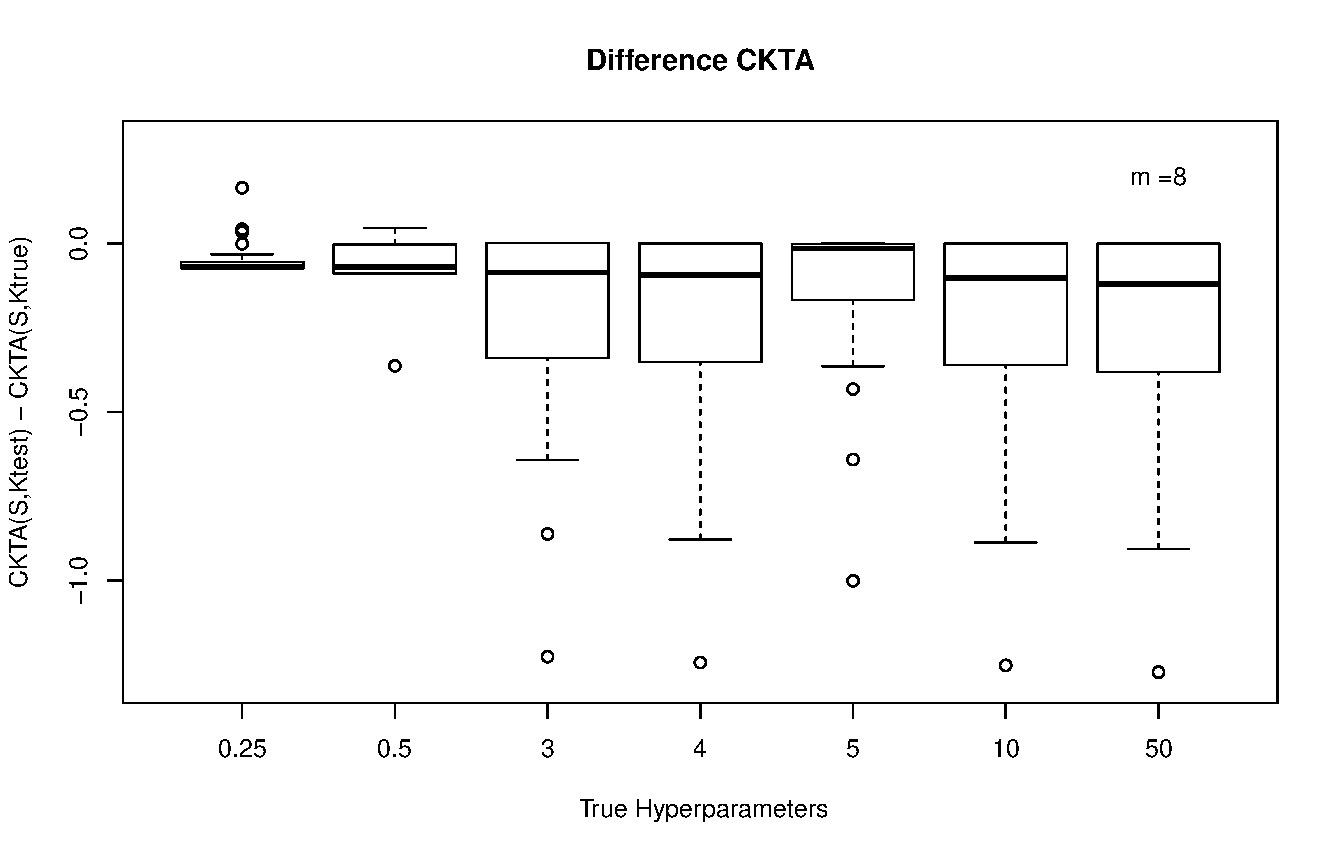
\includegraphics[width=.8\linewidth]{dif_ckta_m_8.pdf}
%  \caption{1a}
  \label{fig:sfig1}
\end{subfigure}


\label{fig1}
\end{figure}

\end{landscape}

\restoregeometry


\newgeometry{left=2.3cm,bottom=0.1cm} 
\begin{landscape}
\begin{figure}
\begin{subfigure}{\textwidth}
  \centering
  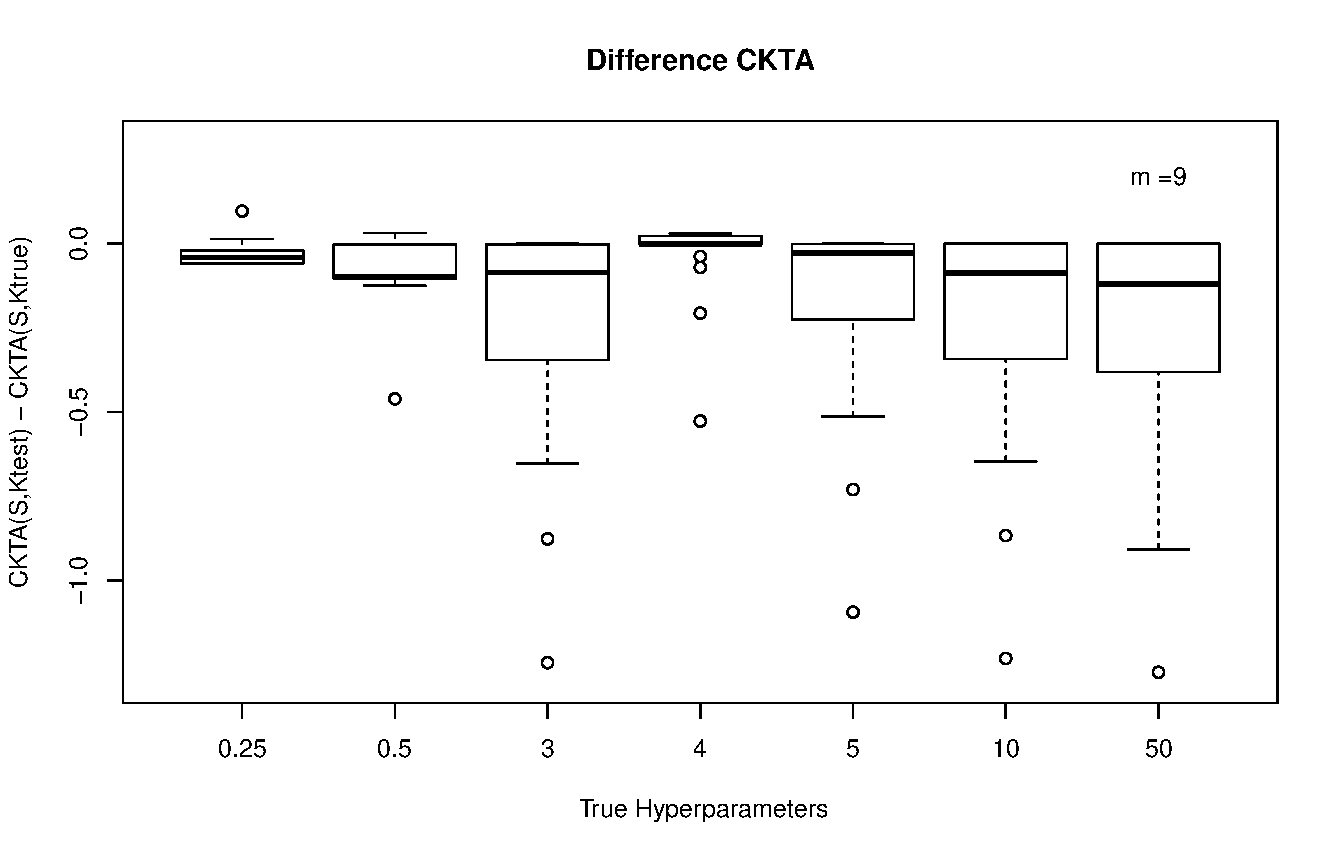
\includegraphics[width=.8\linewidth]{dif_ckta_m_9.pdf}
%  \caption{1a}
  \label{fig:sfig1}
\end{subfigure}%
\begin{subfigure}{\textwidth}
  \centering
  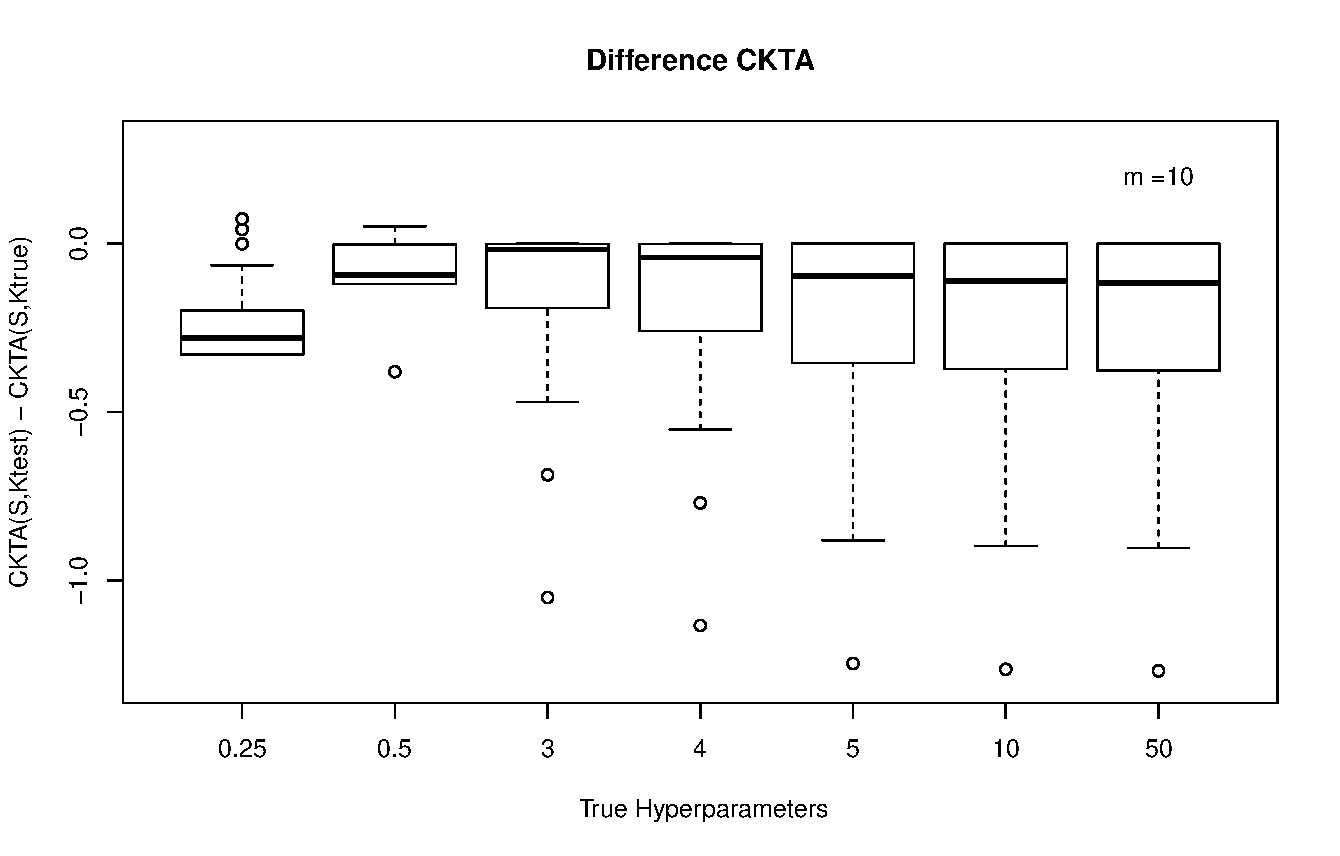
\includegraphics[width=.8\linewidth]{dif_ckta_m_10.pdf}
%  \caption{1b}
  \label{fig:sfig2}
\end{subfigure}
\label{fig1}
\end{figure}

\end{landscape}

\restoregeometry







\end{document}